\lecture{2}{2020-06-11}{Supervised Learning of Behaviours}

\section{Terminología y notación}%
\label{sec:terminología_y_notación}

Las observaciones serán llamadas $o$, las acciones $a$, y la distribución que
calcula las acciones según las observaciones se llamará $\pi_\theta(a|o)$. Donde  $\theta$ son
los parámetros de la función que se tienen que aprender.

Para hacer referencia a que estos valores son secuenciales en el tiempo, se les añade $a$ y $o$
el subíndice $t$ : $a_t, o_t$.

Debajo de las observaciones están los estados. Puede ser que las observaciones
coincidan con el estado del entorno, pero también puede ser que la observación contenga sólo
información incompleta del estado del entorno.\\ Por  ejemplo en un robot que tenga una
cámara, los píxeles que lee la cámara son una consecuencia del estado de las posiciones de todos
los objetos del entorno.

\begin{figure}[htpb]
	\centering
	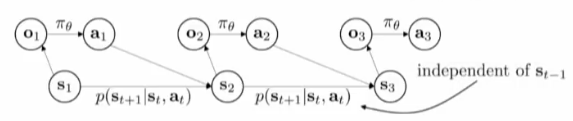
\includegraphics[width=0.8\linewidth]{figures/2020-06-11-131020_573x121_scrot.png}
    \caption{Si se observa $s_1$,  $s_3$ es totalmente independiente de  $s_1$ (Propiedad de
        Markov). Esto no es
    cierto en las observaciones. Por ejemplo si se conoce $o_2$, conocimiento de  $o_1$
también puede ayudar a tomar una mejor decisión.}
\end{figure} 

Los nombre $s_t$ y $a_t$ vienen de Richard Bellman, mientras que en teoría de control, sus
equivalentes $x_t$ (estado) y $u_t$ (acción) viene del ruso.

\section{Imitation Learning}%
\label{sec:imitation_learning}

Si se tiene por ejemplo la tarea de conducción automática, se puede crear un dataset de
observaciones con las acciones de agentes humanos conduciendo y entrenar una política
parametrizada por una red neuronal para que aprenda.

\begin{figure}[htpb]
	\centering
	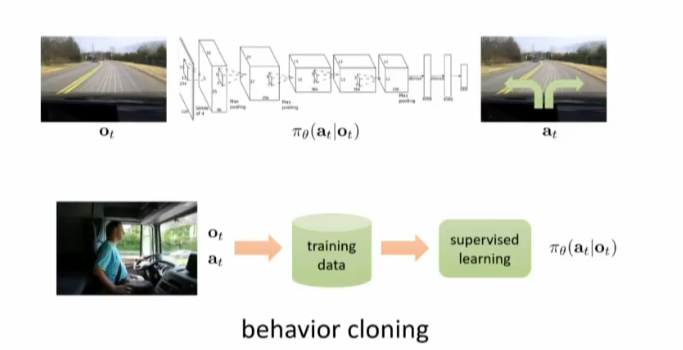
\includegraphics[width=0.8\linewidth]{figures/2020-06-11-131716_683x350_scrot.png}
\end{figure}

Generalmente, si se hace lo que se acaba de explicar, no funciona. Diferentes cosas
pueden ir mal:
\begin{itemize}
    \item Situaciones nunca vistas
    \item Los agentes humanos hacen acciones erróneas
    \item Los agentes humanos pueden tomar acciones basándose en información del pasado.
    \item Se tienen los mismos problemas que en problemas comunes de aprendizaje
        supervisado.
\end{itemize}

\begin{figure}[htpb]
	\centering
	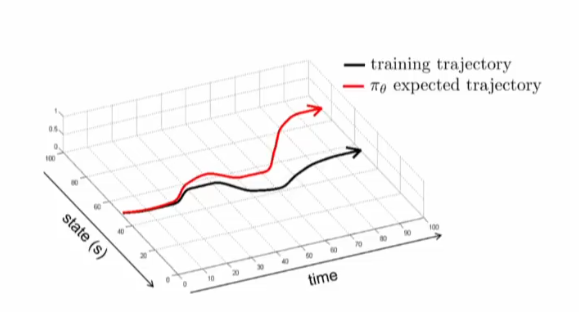
\includegraphics[width=0.8\linewidth]{figures/2020-06-11-132114_579x312_scrot.png}
	\caption{Si se considera una tarea con un estado unidimensional y se entrena un modelo
    para que siga la trayectoria pintada en negro, el algoritmo cometerá errores pequeños que
lo irán alejando cada vez más del conjunto de entrenamiento. Esto hará que cada vez los estados
que vea sean más distintos de los vistos en el entrenamiento, por lo que se cometeran errores
cada vez más grandes y se divergerá de la política deseada.}
\end{figure}

En la práctica, sorprendentemente funciona más o menos (por ejemplo el trabajo de
conducción autónoma de NVIDIA en 2016). 

¿Por qué funciona? Hay dos formas de estabilizar el modelo:
\begin{itemize}
    \item Se añaden tres cámaras: frontal y dos ligeramente a los lados. La frontal se entrena
        normal pero las laterales se entrenan con las acciones modificadas para que se gire el
        volante en la dirección que centre el coche en la trayectoria.
    \item Se puede introducir ruido estadístico para crear varias trayectorias
        parecidas. Lo que evita que el agente diverja en cuanto se aleje de la trayectoria
        original.
\end{itemize}

El problema de Imitation Learning viene de que
$p_{data}(o_t)=p_{\pi_\theta}(o_t)$. Lo que se puede hacer es intentar modificar $p_{data}$
para que se parezca a la política perfecta. Esta es la idea detrás de DAgger.Idealmente este
algoritmo garantiza la solución perfecta dado un tiempo infinito. En la práctica
evidentemente esto no es así.

\begin{algorithm}
    \caption{DAgger: Dataset Aggregation}
    \While{iteraciones deseadas}{
    Entrenar $\pi_\theta(a_t | o_t)$ a partir de datos humanos  $D=\{o_1,a_1,\ldots,o_N,a_N\}$\\
    Ejecutar $\pi_\theta(a_t|o_t)$ para obtener el dataset $D_\pi=\{o_1,\ldots,o_M\}$\\
    Pedir a un humano que decida la acción de cada observación de $D_\pi$\\
    Agregar:  $D \gets D \cup D_\pi$ }
\end{algorithm}

Se podría empezar con una política aleatoria en el principio y también se mantienen las
garantías de convergencia.

Este algoritmo tiene varios problemas:
\begin{itemize}
    \item Se requieren humanos.
    \item Los humanos puede que no elijan las mejores acciones ya que nos somos Markonianos. El
        mundo no es estático como un tablero de ajedrez.
\end{itemize}

\subsection{¿Se puede hacer trabajar Imitation Learning con menos datos?}%
\label{sub:_se_puede_hacer_trabajar_imitation_learning_con_menos_datos_}

\begin{itemize}
    \item DAgger resuelve el problema de la deriva distribucional.
    \item Si se tiene un modelo que es tan bueno que no falla se puede eliminar casi
        completamente esta deriva.
    \item Se tiene que mimetizar comportamientos expertos muy precisamente.
    \item No vale con sobreentrenar.
\end{itemize}

\subsection{¿Por qué podemos fallar al entrenar el experto?}%
\label{sub:_por_qué_podemos_fallar_al_entrenar_el_experto_}

\begin{itemize}
    \item Los humanos no tenemos un comportamiento Markoviano.
    \item Los humanos tenemos un comportamiento multimodal (ánimo, zurdo/diestro, \ldots).
\end{itemize}

Para arreglar lo primero, se puede entrenar una red neuronal que dependa de todas las
observaciones hasta el momento. Por ejemplo una red neuronal recurrente.

\begin{figure}[htpb]
	\centering
	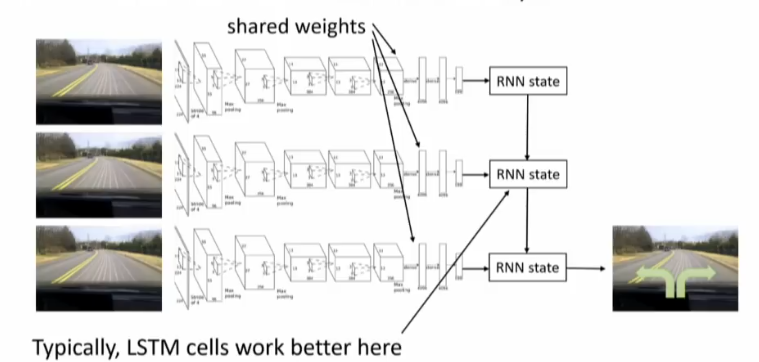
\includegraphics[width=0.8\linewidth]{figures/2020-06-11-135236_759x362_scrot.png}
	\caption{Esquema básico de un controlador con redes recurrentes.}
\end{figure}

Para tratar con lo segundo primero es mejor verlo con un ejemplo. Si queremos rodear un
árbol, podemos elegir por la izquierda o por la derecha ya que ambas son igual de razonables.
Pero una política que sea la media de ambas no sería razonable. Las acciones multimodales en
algunos casos no son un problema. Por ejemplo en el caso de acciones discretas, que se
puede seleccionar con una \textit{softmax}. En el ámbito contínuo esto es más complejo.
Actualmente se suelen usar distribuciones gaussianas y se entrenan con MSE. Hay varias opciones:
\begin{itemize}
    \item Mezclas de gaussianas. La más sencilla pero menos expresiva.
    \item Latent variable models.
    \item Autoreressive discretization.
\end{itemize}

\subsubsection{Mezclas de gaussianas}%
\label{ssub:mezclas_de_gaussianas}

Se usan Mixture Density Networks. Las redes neuronales aprenden los parámetros de las
distribuciones gaussianas. Esto funciona bien con dimensiones bajas. 

\subsubsection{Latent Variable Models}%
\label{ssub:latent_variable_models}

Es la solución más compleja pero la más general. No se cambia la salida de la red. Lo que se
hace es inyectar una entrada adicional al modelo (como por ejemplo un número aleatorio a partir
de una distribución gaussiana). Lo que se pretende es que la red neuronal aprenda a escoger
una de las acciones multimodales a partir de esta entrada inyectada, y es precisamente donde
reside la dificultad de este método.

\begin{figure}[htpb]
	\centering
	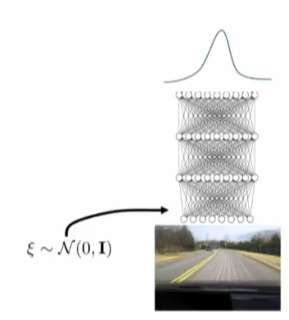
\includegraphics[width=0.4\linewidth]{figures/2020-06-11-140924_289x320_scrot.png}
\end{figure}

Para solventar este problema, existen las siguientes aproximaciones:
\begin{itemize}
    \item Conditional Variational Autoencoder
    \item Normalizing flow / real NVP
    \item Stein variational gradient descent
\end{itemize}

\subsubsection{Autoregressive discretization}%
\label{ssub:autoregressive_discretization}

Se pretende discretizar el espacio de las acciones. Como no es posible simplemente asignar
celdas ya que se tiene el problema de la maldición de la dimensionalidad, lo que se hace es
entrenar la red para que saque la distribución de probabilidades de todas las celdas discretas
de la dimensión primera. Se saca un valor de esa distribución que será el usado en la acción.
A continuación se pasa esa distribución a otra red neuronal que sacará la distribución de la
segunda acción. Se saca el valor de la segunda acción. Seguidamente se pasan las dos
distribuciones de la primera y segunda dimensión a una tercera red para sacar la
distribución de la tercera dimensión, y así sucesivamente.

\begin{figure}[htpb]
	\centering
	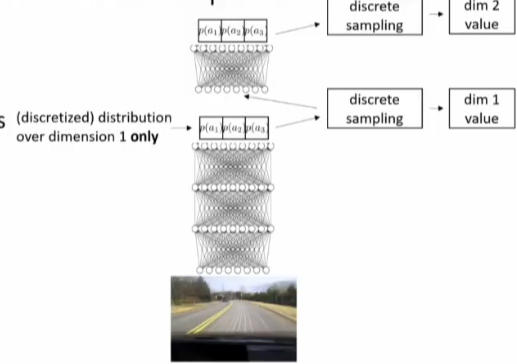
\includegraphics[width=0.8\linewidth]{figures/2020-06-11-141237_517x364_scrot.png}
\end{figure}

Sigue teniendo la desventaja de que los resultados son muy dependientes del tamaño de las
discretizaciones.

\subsection{¿Qué funciones de coste son buenas para Imitation Learning?}%
\label{ssub:_qué_funciones_de_coste_son_buenas_para_imitation_learning_}

\begin{itemize}
    \item $r(s,a) = \log p(a=\pi^*(s) | s)$. Se convierte en coste poniéndole el signo
        negativo (Negative Log Likelihood).
    \item $c(s, a) = \begin{cases}
            0 \textrm{ if } a = \pi^*(s)\\
            1 \textrm{ otherwise }
    \end{cases}$
\end{itemize}

DAgger funciona con ambas.

A continuación se hace un pequeño análisis. $T$ es un tiempo finito, y se considera la función
de recompensa segunda. Se asume que se hace bien en el set de entrenamiento: $\pi_\theta (a \neq
\pi^*(s)|s) \leq \epsilon \;\forall\; s \in D_{train}$.o

\begin{align}
    E\left[\sum_t c(s_t, a_t)\right] \leq \epsilon T +
    (1-\epsilon)(\epsilon(T-1)+(1-\epsilon)(\ldots))
\end{align}

Esto es así porque si se falla en el primer paso, en el resto también se falla ($\epsilon
T$), si en el primer paso pero en el segundo no, se tiene
$(1-\epsilon)(\epsilon(T-1))$ y así sucesivamente.

Lo que significa que la función de coste será $O(\epsilon T^2)$, lo que es muy malo ya que el
coste aumenta cuadráticamente con la duración de la trayectoria.

La asunción de que solo podemos coger estados de  $D_train$ es muy débil. Se sabe que los
modelos de aprendizaje supervisados son capaces de generalizar, dado un número grande de
datos. Por lo que podremos asumir que el modelo seguirá funcionando mientras reciba estados que
provengan de la distribución de datos de los que fue entrenado. Por lo que ahora: $\pi_\theta (a
\neq \pi^*(s)|s) \leq \epsilon \textrm{ para } s \sim p_{train}(s)$.

Por lo que ahora:
\begin{align}
    E\left[\sum_t c(s_t, a_t)\right] \leq \epsilon T
\end{align}

Y la función de coste estará acotada por $O(\epsilon T)$ y será razonable usar Imitation
Learning.
